\chapter{Leader-follower networks}


\begin{description}
    \item[Leader-follower network] \marginnote{Leader-follower network}
        Consider agents partitioned into $N_f$ followers and $N-N_f$ leaders.
        
        The state vector can be partitioned as:
        \[ \x = \begin{bmatrix} \x_f \\ \x_l \end{bmatrix} \]
        where $\x_f \in \mathbb{R}^{N_f}$ are the followers' states and $\x_l \in \mathbb{R}^{N-N_f}$ the leaders'.
        
        The Laplacian can also be partitioned as:
        \[
            \lap = \begin{bmatrix} \lap_f & \lap_{fl} \\ \lap_{fl}^T & \lap_l \end{bmatrix}
        \]
        where $\lap_f$ is the followers' Laplacian, $\lap_l$ the leaders', and $\lap_{fl}$ is the part in common.

        Assume that leaders and followers run the same Laplacian-based distributed control law (i.e., an normal averaging system), the system can be formulated as:
        \[
            \begin{bmatrix} \dot{\x}_f(t) \\ \dot{\x}_l(t) \end{bmatrix} =
            - \begin{bmatrix} \lap_f & \lap_{fl} \\ \lap_{fl}^T & \lap_l \end{bmatrix}
            \begin{bmatrix} \x_f(t) \\ \x_l(t) \end{bmatrix}
        \]

        \begin{example}
            Consider a path graph with four nodes:
            \[ 0 \leftrightarrow 1 \leftrightarrow 2 \leftrightarrow (3) \]
            The nodes $0, 1, 2$ are followers and $3$ is a leader. The system is:
            \[
                \begin{bmatrix}
                    \dot{x}_1(t) \\ \dot{x}_2(t) \\ \dot{x}_3(t) \\ \dot{x}_4(t)
                \end{bmatrix} = 
                \begin{bmatrix}
                    \begin{tabular}{ccc|c}
                        1   & -1    & 0     & 0     \\
                        -1  & 2     & -1    & 0     \\
                        0   & -1    & 2    & -1    \\
                        \hline
                        0   & 0     & -1    & 1     \\
                    \end{tabular}
                \end{bmatrix}
                \begin{bmatrix}
                    x_1(t) \\ x_2(t) \\ x_3(t) \\ x_4(t)
                \end{bmatrix}
            \]
    \end{example}

\end{description}



\section{Containment}

\begin{description}
    \item[Containment] \marginnote{Containment}
        Task where leaders are stationary and the goal is to drive followers within the convex hull enclosing the leaders. Followers can communicate with agents of any type while leaders do not communicate.

        \begin{figure}[H]
            \centering
            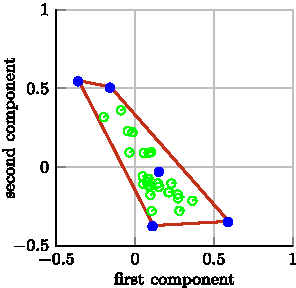
\includegraphics[width=0.3\linewidth]{./img/_containment.pdf}
        \end{figure}

    \item[Containment control law] \marginnote{Containment control law}
        Given $N_f$ followers and $N-N_f$ leaders, the control law to solve the containment task have:
        \begin{itemize}
            \item Followers running Laplacian dynamics.
            \item Leaders being stationary.
        \end{itemize}

        The system is:
        \[
            \begin{aligned}
                \dot{x}_i(t) &= - \sum_{j \in \mathcal{N}_i} a_{ij} \big( x_i(t) - x_j(t) \big) & & \forall i \in \{ 1, \dots, N_f \} \\
                \dot{x}_i(t) &= 0 & & \forall i \in \{ N_f + 1, \dots, N \}
            \end{aligned}
        \]
        In matrix form, it becomes:
        \[
            \begin{split}
                \dot{\x}(t) &= - \lap \x(t) \\
                \begin{bmatrix} \dot{\x}_f(t) \\ \dot{\x}_l(t) \end{bmatrix} &=
                - \begin{bmatrix} \lap_f & \lap_{fl} \\ 0 & 0 \end{bmatrix}
                \begin{bmatrix} \x_f(t) \\ \x_l(t) \end{bmatrix} \\
                \dot{\x}_f(t) &= - \lap_f \x_f(t) - \lap_{fl} \x_l
            \end{split}
        \]
        where $\lap_f$ can be seen as the state matrix and
        $\lap_{fl}$ as the input matrix. The input $\x_l = \x_l(0) = \x_l(t)$ is constant.
\end{description}

\begin{lemma} \phantomsection\label{th:laplacian_positive_definite}
    If the interaction graph $G$ between leaders and followers is undirected and connected, then the followers' Laplacian $\lap_f$ is positive definite.
    
    \begin{proof}
        We need to prove that:
        \[ \x_f^T \lap_f \x_f > 0 \quad \forall \x_f \neq 0 \]

        As $G$ is undirected, it holds that:
        \begin{itemize}
            \item The complete Laplacian $\lap$ is symmetric and thus have real-valued eigenvalues.
            \item By \Cref{th:weighted_laplacian_eigenvalues}, all its non-zero eigenvalues are positive.
            \item By \Cref{th:connected_simple_eigenvalue}, as $G$ is connected, the eigenvalue $\lambda=0$ is simple.
        \end{itemize}
        Therefore:
        \begin{itemize}
            \item $\x^T \lap \x \geq 0$ as all eigenvalues are non-negative.
            \item $\x^T \lap \x = 0 \iff \vec{x} = \alpha\vec{1}$ for $\alpha \in \mathbb{R}$, as $\lambda=0$ is simple.
        \end{itemize}

        The following two arguments can be made:
        \begin{enumerate}
            \item By choosing $\bar{\x} = \begin{bmatrix} \x_f & 0 \end{bmatrix}^T$, it holds that:
                \[
                    \begin{aligned}
                        \bar{\x}^T \lap \bar{\x} &\geq 0 & & \forall \bar{\x} \\
                        \begin{bmatrix} \x_f & 0 \end{bmatrix}
                        \begin{bmatrix}
                            \lap_f & \lap_{fl} \\
                            \lap_{fl}^T & \lap_{l} \\
                        \end{bmatrix}
                        \begin{bmatrix} \x_f \\ 0 \end{bmatrix} &\geq 0 & & \forall \x_f \\
                        \x_f^T \lap_f \x_f &\geq 0 & & \forall \x_f
                    \end{aligned}
                \]
            \item The only case when $\x^T \lap \x = 0$ for $\x \neq 0$ is with $\x = \alpha\vec{1}$ for $\alpha \neq 0$. As $\forall \x_f: \bar{\x} \neq \alpha\vec{1}$, it holds that $\forall \x_f: \x_f^T \lap_f \x_f \neq 0$.
        \end{enumerate}
        Therefore, $\lap_f$ is positive definite as $\forall \x_f \neq 0: \x_f^T \lap_f \x_f > 0$.
    \end{proof}
\end{lemma}

\begin{lemma} \phantomsection\label{th:laplacian_globally_exponentially_stable}
    It holds that $\dot{\x}_f = -\lap_f \x_f$ is globally exponentially stable (i.e., converges to $0$ exponentially).

    \begin{proof}
        As $\lap_f$ is symmetric and positive definite by \Cref{th:laplacian_positive_definite}, its eigenvalues are real and positive. Therefore, $-\lap_f$ have real and negative eigenvalues, which is the condition of a globally exponentially stable behavior.
    \end{proof}
\end{lemma}

\begin{theorem}[Containment optimality] \phantomsection\label{th:containment_optimality} \marginnote{Containment optimality}
    Given a leader-follower network such that:
    \begin{itemize}
        \item Followers run Laplacian dynamics,
        \item Leaders are stationary,
        \item The interaction graph $G$ is fixed, undirected, and connected.
    \end{itemize}
    It holds that all followers asymptotically converge to a state (not necessarily the same) within the convex hull containing the leaders.

    \begin{proof}
        The proof is done in two parts:
        \begin{descriptionlist}
            \item[Unique globally asymptotically stable equilibrium] 
                We want to prove that the followers' state $\x_f(t)$ converges to some value $\x_{f,E}$ for any initial state. The equilibrium can be found by solving:
                \[ 0 = -\lap_f \x_{f,E} - \lap_{fl} \x_l \]
                where $\dot{\x}_f = 0$ (i.e., reached convergence) and $\x_{f,E}$ is the equilibrium state.

                By \Cref{th:laplacian_positive_definite}, $\lap_f$ is positive definite and thus invertible, therefore, we have that:
                \[  \x_{f,E} = -\lap_f^{-1} \lap_{fl} \x_l \]

                Let $\vec{e}(t) = \x_f(t) - \x_{f,E}$ (intuitively, the distance to equilibrium). As the rate of change of $\vec{e}(t)$ depends only on $\x_f(t)$ (i.e., $\dot{\vec{e}}(t) = \dot{\x}_f(t)$), we have that:
                \[
                    \begin{split}
                        \dot{\vec{e}}(t) &= \dot{\x}_f(t) \\
                            &= -\lap_f \x_f(t) - \lap_{fl} \x_l \\
                            &= -\lap_f (\vec{e}(t) + \x_{f,E}) - \lap_{fl} \x_l \\
                            &= -\lap_f \vec{e}(t) + \cancel{\lap_f \lap_f^{-1} \lap_{fl} \x_l} - \cancel{\lap_{fl} \x_l} \\
                    \end{split}
                \]
                
                \begin{lemma} \phantomsection\label{th:lti_stability_equilib_traj}
                    Any equilibrium or trajectory based on an LTI system enjoys the same stability property of that system.
                \end{lemma}

                As \Cref{th:laplacian_globally_exponentially_stable} states that $\dot{\x}_f = -\lap_f \x_f$ is globally asymptotically stable, by \Cref{th:lti_stability_equilib_traj}, it holds that $\dot{\vec{e}}(t) = -\lap_f \vec{e}(t)$ is also a globally asymptotically stable system and $\x_{f,E}$ is the unique globally stable equilibrium of the followers' dynamics.

            \item[Equilibrium within convex hull] 
                We want to prove that each element of $\x_{f,E}$ falls within the convex hull of the leaders.

                For simplicity, let us denote the states vector as $\x_E = \begin{bmatrix} \x_{f,E} & \x_l \end{bmatrix}^T$ and its $i$-th component as $x_{E,i}$.

                The dynamics at convergence of the $i$-th follower is:
                \[ 0 = - \sum_{j=1}^N a_{ij} (x_{E,i} - x_{E,j}) \quad \forall i \in \{ 1, \dots, N_f \} \]
                Therefore, we have that:
                \[
                    \begin{aligned}
                        \left( \sum_{j=1}^N a_{ij} \right) x_{E,i} &= \sum_{j=1}^N a_{ij} x_{E,j} & & \forall i \in \{ 1, \dots, N_f \} \\
                        x_{E,i} &= \sum_{j=1}^N \frac{a_{ij}}{\sum_{k=1}^N a_{ik}} x_{E,j} & & \forall i \in \{ 1, \dots, N_f \} \\
                    \end{aligned}
                \]
                As $\frac{a_{ij}}{\sum_{k=1}^N a_{ik}}$ define a convex combination (i.e., sum of all of them is $1$), each follower's equilibrium $x_{E,i}$ belongs to the convex hull of all the other agents (both leaders and followers). As leaders are stationary, they are not affected by this constraint and it can be concluded that followers' equilibria fall within the convex hull of the leaders.
        \end{descriptionlist}
    \end{proof}
\end{theorem}

\begin{remark}[Leader-follower containment weakness]
    The final part of the proof of \Cref{th:containment_optimality} also shows that if there is an adversarial follower that does not change its state, all others will converge towards it.
\end{remark}


\section{Containment with non-static leaders}

\begin{description}
    \item[Containment with non-static leaders] \marginnote{Containment with non-static leaders}
        Containment problem where leaders' dynamics is a non-zero constant (i.e., they also move):
        \[
            \begin{aligned}
                \dot{\x}_f(t) &= -\lap_f \x_f(t) - \lap_{fl} \x_l(t) \quad & \x_f(0) &= \x_f^{(0)} \\
                \dot{\x}_l(t) &= \vec{v}_0 \quad & \x_l(0) &= \x_l^{(0)} \\
            \end{aligned}
        \]
        where $\vec{v}_0$ is the leaders' velocity.
\end{description}

\begin{theorem}[Containment with non-static leaders non-equilibrium]
    Naive containment with non-static leaders do not have an equilibrium.

    \begin{proof}
        Ideally, the equilibria for followers' and leader's dynamics are:
        \[
            \begin{split}
                0 &= -\lap_f \x_{f,E} - \lap_{fl} \x_{l,E} \\
                0 &= \vec{v}_0
            \end{split}
        \]

        Let's define the containment error (can also be seen as the error to reach the followers' equilibrium) as:
        \[
            \vec{e}(t) = \lap_f \x_f(t) + \lap_{fl} \x_l(t)
        \]
        Its dynamics depends on the ones of the followers' and leaders':
        \[
            \begin{split}
                \dot{\vec{e}}(t) &= \lap_f \dot{\x}_f(t) + \lap_{fl} \dot{\x}_l(t) \\
                &= \lap_f (- \lap_f \x_f(t) - \lap_{fl} \x_l(t)) + \lap_{fl} \vec{v}_0 \\
                &= - \lap_f \vec{e}(t) + \lap_{fl} \vec{v}_0
            \end{split}
        \]
        
        By inspecting the value of the containment error $\vec{e}(t)$ when it reaches equilibrium we have that:
        \[
            \begin{split}
                0 &= \dot{\vec{e}}(t) \\
                \iff 0 &= - \lap_f \vec{e}(t) + \lap_{fl} \vec{v}_0 \\
                \iff \vec{e}(t) &= \lap_f^{-1} \lap_{fl} \vec{v}_0 \\
            \end{split}
        \]
        
        There are two cases:
        \[
            \vec{e}(t) = \begin{cases}
                0 & \text{if $\vec{v}_0 = 0$ (i.e., same case of \Cref{th:containment_optimality})} \\
                \lap_f^{-1} \lap_{fl} \vec{v}_0 & \text{if $\vec{v}_0 \neq 0$} \\
            \end{cases}
        \]

        Therefore, when leaders are non-static, the containment error converges to a non-zero constant. Thus, followers' equilibrium is never reached (i.e., they keep moving) and the containment problem cannot be solved.
    \end{proof}
\end{theorem}



\section{Containment with non-static leaders and integral action}

\begin{description}
    \item[Containment with non-static leaders and integral action] \marginnote{Containment with non-static leaders and integral action}
        Leader-follower dynamics defined as:
        \[
            \begin{aligned}
                \dot{\x}_f(t) &= -\lap_f \x_f(t) - \lap_{fl} \x_l(t) + \vec{u}_f(t) \quad & \x_f(0) &= \x_f^{(0)} \\
                \dot{\x}_l(t) &= \vec{v}_0 \quad & \x_l(0) &= \x_l^{(0)} \\
            \end{aligned}
        \]
        where $\vec{u}_f(t)$ is a distributed control action (can be seen as a correction) that processes the containment error $\vec{e}(t)$. It is composed of a proportional controller (i.e., value proportional to the error) and an integral controller (i.e., value proportional to the integral to the error):
        \[
            \begin{split}
                \vec{u}_f(t) &= \matr{K}_P \vec{e}(t) + \matr{K}_I \int_{0}^{t} \vec{e}(\tau) \,d\tau
            \end{split}
        \]
        where $\matr{K}_P$ and $\matr{K}_I$ are coefficients for the proportional and integral controller, respectively.
        
        By defining a proxy $\xi$ for the integral of the error (i.e., sort of accumulator) as follows:
        \[
            \begin{split}
                \dot{\xi}(t) &= \vec{e}(t) \\
                    &= \lap_f \vec{x}(t) + \lap_{fl} \x_l(t) \qquad \xi(0) = \xi^{(0)}
            \end{split}
        \]
        The control action can be defined as:
        \[
            \vec{u}_f(t) = \matr{K}_P \vec{e}(t) + \matr{K}_I \xi(t)
        \]

        In the simplest case, $\vec{u}_f(t)$ is a pure integral control where $\matr{K}_I = -\kappa_I \matr{I}, \kappa_I>0$ is a sparse matrix (e.g., diagonal) and $\matr{K}_P = 0$. The overall system can be defined in matrix form as:
        \[
            \begin{bmatrix}
                \dot{\x}_f(t) \\ \dot{\x}_l(t) \\ \dot{\xi}(t)
            \end{bmatrix}
            =
            \begin{bmatrix}
                -\lap_f & -\lap_{fl} & \matr{K}_I \\
                0 & 0 & 0 \\
                \lap_f & \lap_{fl} & 0 
            \end{bmatrix}
            \begin{bmatrix}
                \x_f(t) \\ \x_l(t) \\ \xi(t)
            \end{bmatrix}
            +
            \begin{bmatrix}
                0 \\ \matr{I} \\ 0
            \end{bmatrix}
            \vec{v}_0
        \]
\end{description}

\begin{remark}
    The value of this formulation of the control action for an agent $i$ is:
    \[
        \begin{split}
            u_{F_i}(t) = \kappa_I \xi_i(t) \\
        \end{split}
    \]
    It can be seen that it is computable as a distributed system as $\kappa_I$ is constant and $\xi_i(t)$ is based on the Laplacian (i.e., it is sufficient to look up the neighbors' states).
\end{remark}

\begin{theorem}[Containment with non-static leaders and integral action optimality]
    With the integral action, containment with non-static leaders converges to a valid solution.
\end{theorem}



\section{Containment with discrete-time}

\begin{description}
    \item[Containment with discrete-time] \marginnote{Containment with discrete-time}
        Containment can be discretized using the forward-Eurler discretization. Its dynamics is defined as:
        \[
            \begin{aligned}
                \dot{\x}_i(t) &= - \sum_{j \in \mathcal{N}_i} a_{ij} (x_i(t) - x_j(t)) & & \forall i \in \{1, \dots, N_f\} \\
                \dot{\x}_i(t) &= 0 & & \forall i \in \{N_f+1, \dots, N\}
            \end{aligned}
        \]
        And the followers' states are sampled with a time-step $\varepsilon > 0$ while the leaders' is constant:
        \[
            \begin{split}
                x_i^{k+1} &= \left.x_i(t)\right|_{t=(k+1)\varepsilon} \\
                &= x_i^k + \varepsilon \left.\dot{x}_i(t)\right|_{t=k\varepsilon} \\
                &= \left( 1 - \varepsilon\sum_{j \in \mathcal{N}_i} a_{ij} \right) x_i^{k} + \varepsilon \sum_{j \in \mathcal{N}_i} a_{ij} x_j^k \qquad \forall i \in \{ 1, \dots, N_f \} \\
                x_i^{k+1} &= x_i^k \qquad \forall i \in \{ N_f+1, \dots, N \}
            \end{split}
        \]
        In matrix form, it can be defined as:
        \[
            \begin{bmatrix}
                \x_f^{k+1} \\ \x_l^{k+1} 
            \end{bmatrix}
            =
            \begin{bmatrix}
                \matr{I} - \varepsilon \lap_f & -\varepsilon \lap_{fl} \\
                0 & \matr{I}
            \end{bmatrix}
            \begin{bmatrix}
                \x_f^k \\ \x_l^k
            \end{bmatrix}
        \]
\end{description}



\section{Containment with multivariate states}

\begin{description}
    \item[Containment with multivariate states] \marginnote{Containment with multivariate states} 
        With multivariate states, it can be shown that the dynamics is described as:
        \[
            \dot{\x}(t) = - \lap \otimes \matr{I}_d \x(t)
        \]
        where $\otimes$ is the Kronecker product.
\end{description}